\documentclass[a4paper, 12pt]{article}
\usepackage[utf8]{inputenc}
\usepackage[T2A]{fontenc}
\usepackage[english, russian]{babel} 
\usepackage{amscd, amsmath, amssymb, amsthm, enumerate, indentfirst, longtable, ifthen} % addlibrary rom mathematic 
\usepackage{ragged2e}
\usepackage{microtype}
\usepackage{indentfirst}
\usepackage{setspace}
\usepackage{pgfplots} %graf create
\usepackage{graphicx,xcolor} % графика для svg
%\usepackage{pdfpages}

\setstretch{1.15} % interval 
% PGFPlots setting
\pgfplotsset{compat=1.9}

% picture 
\RequirePackage{caption}
\DeclareCaptionLabelSeparator{defffis}{.}
\captionsetup{justification=centering,labelsep=defffis}
\usepackage{graphicx}
\graphicspath{{fig/}}
\DeclareGraphicsExtensions{.png,}
% end picture 

\usepackage{geometry}
\geometry{
 	tmargin=15mm,         % Up 
 	bmargin=15mm,         % Down 
 	lmargin=15mm,         % left поле
 	rmargin=15mm,         % right  
}

% new command 
\newcommand{\jj}{\righthyphenmin=20 \justifying}
% opening
\date{25 апреля, 2018}
\title{Распределение вознаграждения между узлами сети блокчейн}
\author{noise@sumus.team, engi@sumus.team}

\begin{document}

\maketitle

\begin{abstract}
Предлагается подход к оценке возможности равноправного получения узлами блокчейна вознаграждения за закрытие блоков. Для описания потоков транзакций и закрытия блоков применяется теория случайных процессов. Приводится пример получения узлами вознаграждений, незначительно различающихся по величине и являющихся значениями нормально распределённой случайной величины.
%%Правило мотивации постоянного подключения узла к сети \dots\dots
\end{abstract}

\section{Введение}\addcontentsline{toc}{section}{Введение}

Сначала рассмотрим  вопрос о распределении вознаграждения между узлами для случая, когда все узлы из $B_n$ постоянно присутствуют в сети. Тогда они равноправны в том смысле, что вероятность получения любым  узлом в произвольный момент $t$ закрытия блока вознаграждения в интервале, величина которого зафиксирована на этот момент, зависит только от величины интервала и количества узлов $n$ \cite{sumus180427}.

\section{Основные положения и допущения}\addcontentsline{toc}{section}{Основные положения и допущения}

Будем считать величину вознаграждения $\zeta$ функцией времени $t$, где в некоторый момент $t_k$, соответствующий проведению отдельной транзакции, $\zeta(t_k)$ принимает значение равное $\zeta$, ``начисленному'' за эту транзакцию \cite{budish180605}. Пусть $T$ --- счётное множество значений всех $t_k$, в которые осуществляются транзакции, $k=1,2,\dots\;\;$. Множество значений этой функции обозначим  $\Psi$. Таким образом, $\zeta(t_k)$ есть решетчатая неотрицательная функция, заданная на счётном множестве $T$. Поскольку $\zeta$ меняется по закону, который можно установить только статистическими методами, то положим, что $\zeta(t_k)$ есть решетчатая случайная функция, или, другими словами, дискретный случайный процесс. Вообще говоря, этот процесс может быть нестационарным, но при этом следует допустить его эргодичность и слабую коррелированность. Также будем считать, что у этого процесса есть математическое ожидание и дисперсия. Пусть плотность распределения этого процесса есть  $f(\zeta,t)$, где $t \in T$, $\zeta \in \Psi$. Функция $f$ не менее чем непрерывна по $\zeta$, а значит $\zeta(t_k)$ при фиксированном $t_k$ является непрерывной случайной величиной. У $\zeta(t_k)$ есть математическое ожидание и дисперсия \cite{birkhoff1931}.

Пусть также имеет место независимый  от $\zeta$ процесс закрытия блоков, который в данном случае можно представить как дискретный случайный процесс $g(t_m)$, значениями которого являются номера мастер-узлов $j_{\widehat{k}}$, определяемые в моменты  $t_{m} \in [t_{m-1}', t_{m}')$, $m=1,2\dots$ , где $t_{m}'$ -- момент закрытия блока номер $m$, $t_0'$ -- начальный момент работы сети. Процесс $g(t_m)$ -- стационарный с равномерным распределением дискретной случайной величины $j_{\widehat k}$,  $1 \leq j_{\widehat k} \leq N $. Счётное множество всех значений $t_m$ обозначим $T^*$.

\section{Обоснование нормального распределения вознаграждения между постоянно подключёнными узлами}\addcontentsline{toc}{section}{Основание нормального распределения вознаграждения между постоянно подключёнными узлами}

В момент времени $t_m$ закрытия блока номер $m$ мастер-узел  с номером $j_{\widehat{k}}$ получает всю накопленную к этому моменту $\Delta \zeta_{\Sigma}$, которую будем считать равной
\begin{equation} % (1)
	\Delta \zeta _\Sigma ( t_{m} ^{'} ) = \sum\limits _{k = k _{m-1}} ^{k_m} \zeta(t_k)
	\label{equation:randomprocess}
\end{equation}
где $k_{m-1}$ --- номер момента $t_{k_{m-1}}$, ближайшего к $t_{m-1}^{'}$ справа, а $k_m$ --- номер момента $t_{k_m}$, ближайшего к $t_{m}^{'}$ слева.

Поскольку для $\forall {k}, m : t_k - t_{k-1} \ll t_{m}^{'}-t_{m-1}{'}$, то каждое значение случайной функции $\Delta \zeta_{\Sigma} (t_{m}^{'}) $ является суммой большого числа случайных величин и согласно закону больших чисел (при соблюдении условий, указанных выше), имеет распределение близкое к нормальному \cite{lehmann060330}
	
\begin{equation} % (2)
	P((\Delta \zeta_{\Sigma} < a), t) \approx \Phi (a, t)
\end{equation}
а значит, $\Delta \zeta _\Sigma ( t_{m} ^{'} )$ при произвольных, но подобных друг-другу при любых $k$ функциях плотности $f(\zeta,t_k)$, с достаточной точностью является нормальным дискретным случайным процессом \cite{sunkolodas2010}. 

Таким образом, каждый из $n$ узлов может в момент $t_{m}$ стать мастер-узлом с вероятностью $\displaystyle \frac{1}{n}$ и в соответствующий момент $t_{m}^{'}$ получить $\Delta \zeta_{\Sigma} (t_{m}^{'})$, например, в интервале $(M_{\Delta \zeta_{\Sigma}} - 3 \sigma_{\Delta \zeta_{\Sigma}} , M_{\Delta \zeta_{\Sigma}}+3\sigma_{\Delta \zeta_{\Sigma}})$, с вероятностью $\approx {0,997}$, где $M_{\Delta \zeta_{\Sigma}}$ и $\sigma_{\Delta \zeta_{\Sigma}}$ --- математическое ожидание и среднеквадратическое отклонение случайного процесса (\ref{equation:randomprocess}) в момент времени  $t_{m}^{'}$.
	
В результате, в момент $t_{m}^{'}$ каждый из $n$ узлов получает указанное вознаграждение с вероятностью $\displaystyle \frac{0,997}{n}$. Уменьшение интервала значений $\Delta \zeta_{\Sigma} (t_{m}^{'})$, например, в полтора раза приводит к незначительному изменению указанной вероятности.
	
Приведённые выше результаты справедливы при достаточно длительных реализациях случайных процессов, т.е. при $m \gg n$ и их эргодичности.

\section{Пример}\addcontentsline{toc}{section}{Пример}
Покажем, что при способе вознаграждения узлов, описанном выше, эти вознаграждения будут распределены по нормальному закону. Рассмотрим в качестве $\zeta(t_k)$ дискретный случайный процесс, значениями которого являются вознаграждения за одиночные транзакции в системе БИТКОЙН \cite{nakamoto2009}. На основе этого процесса, вычисляются по формуле (\ref{equation:randomprocess}) значения второго дискретного случайного процесса, значениями которого являются вознаграждения $\Delta\zeta_\Sigma$ каждому мастер-узлу, закрывшему блок. На временном интервале от 18.02.2017 до 13.12.2018 процесс $\Delta\zeta_\Sigma$ принимает $10^5$ значений, среди которых наибольшим является 2,0 BTC. Именно этот процесс должен иметь нормальное распределение. Разделим $10^5$ значений этого процесса, упорядоченных по времени, на $10$ кусков, в каждом из которых будет по $10^4$ значений $\Delta\zeta_\Sigma(t_m^{'})$. Таким образом, получены $10$ реализаций исследуемого случайного процесса, в каждом из которых по $10^4$ значений $\Delta\zeta_\Sigma$. Эта операция справедлива, если процесс эргодический \cite{birkhoff1931}. Реализацией № $i$, $i=1,\dots,10$ будем обозначать $\Delta\zeta(t_j)$, где при фиксированном $i$ индекс $j$ ``пробегает'' значения от $1$ до $10^4$. Сечением №$j$ случайного процесса $\Delta\zeta_\Sigma(t_j)$ будет множество  значений $\Delta\zeta_{\Sigma_i}$ при фиксированном $j$ и $i=1,\dots,10$.
	
В произвольно взятом $j$-том сечении будет $10^4$ значений случайной величины $\Delta\zeta_{\Sigma_j}$. Разобьём отрезок $[\min \Delta\zeta_{\Sigma_j}, \max \Delta\zeta_{\Sigma_j}]$ на $r$ одинаковых отрезков (в нашем случае $r=10$). Откладывая по оси абсцисс значения случайной величины $\Delta\zeta_{\Sigma_j}$, а над каждым из $r$ отрезков откладывая по оси ординат количество значений $\Delta\zeta_{\Sigma_j}$ попавших в этот отрезок, получим график, показанный на рис.~\ref{figure:histogram}. После его нормировки делением значений решетчатой функции на $10^4$ получим так называемый ряд распределения случайной величины, значения которой равны средним значениям $\Delta\zeta_{\Sigma_j}$ по каждому из $r$ отрезков разбиения отрезка $[\min \Delta\zeta_{\Sigma_j}, \max \Delta\zeta_{\Sigma_j}]$ (мы полагаем, что на каждом из $r$ отрезков случайная величина $\Delta\zeta_{\Sigma_j}$ принимает практически одни и те же значения). Ряд распределения для дискретных случайных величин является аналогом плотности распределения для непрерывных случайных величин. Нетрудно видеть, что огибающая графика решетчатой функции на рис.~\ref{figure:histogram} будет гауссовой кривой. По ряду распределения нетрудно построить функцию распределения, которая будет кусочно-постоянным приближением функции Лапласа.

Таким образом, экспериментально подтверждено, что вознаграждение за закрытие блока есть нормально распределённая случайная величина, являющаяся функцией времени, другими словами нормальным дискретным случайным процессом.
 
\begin{figure}[htp] 
	\centering
	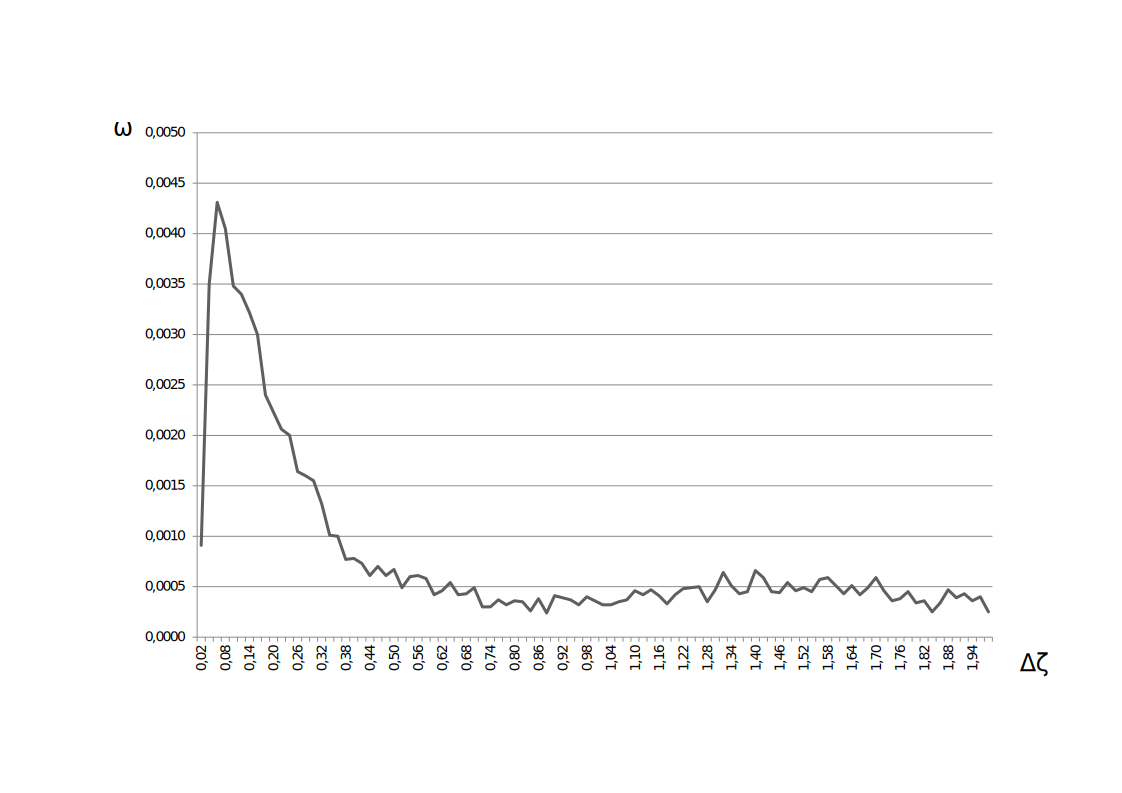
\includegraphics[scale=0.5]{fig/histogram_snp10_sns1_mn1_mx200000000.pdf}
	\caption{\; Экспериментальная кривая плотности распределения вознаграждения между узлами.}
	\label{figure:histogram} 
\end{figure}  
 
\section{Распределение вознаграждения между узлами, не подключёнными постоянно}\addcontentsline{toc}{section}{Распределение вознаграждения между узлами, подключёнными не постоянно}
Рассмотрим теперь вопрос распределения $\zeta$ между узлами для случая, когда не все узлы из $B_n$ постоянно присутствуют в сети. Это означает, что есть некоторое фиксированное подмножество узлов $B_{\widetilde{n}} \subseteq B_n $, $\widetilde{n} \leq n$ (считаем, что $\widetilde{n} < n/3$ ) такое, что для любого узла из $B_{\widetilde{n}}$ справедливо следующее: пусть этот узел  выбирался мастер-узлом $\overline m < m$ раз на отрезке $t \in [t'_0, t_m^*)$, но принял задачу по закрытию блока только $\widetilde{m}$ раз $(\widetilde{m} < \overline{m})$. Тогда за закрытие текущего блока
%, выбор эскорта которого осуществлён в момент $t_{m}^{*}$, этот 
мастер узел получит вознаграждение 
\begin{equation} % (3)
	\gamma_{m} =  \frac{\widetilde{m}}{\overline m} \Delta \zeta_{\Sigma} (t_{m}^{'})  
	\label{equation:for1} 
\end{equation}
%
остаток
%
\begin{equation} % (4)
	\frac{\overline m -\widetilde{m}}{\overline m} \Delta \zeta_{\Sigma} (t_{m}^{'})  
	\label{equation:for2}
\end{equation}
суммируется в дальнейшем с $\Delta \zeta_{\Sigma} (t_{m+1}^{'})$. Можно сказать, что предложено правило мотивации постоянного подключения узла к сети.

В силу независимости процесса включения/отключения узла в сети от других случайных процессов, упомянутых выше, и естественном предположении о стационарности и равномерности распределения номеров $\widetilde{n}$ отключаемых узлов, можно утверждать, что введение ``мотивирующих'' коэффициентов  $\displaystyle M = \frac{\: \widetilde{m}\:}{\overline m}$, и перенос остатков не приведут к изменению классификации случайных процессов, используемых в этой задаче. 

Вероятность того, что в произвольный момент $t_m$ определения нового мастер-узла им станет непостоянно подключенный узел из $B_{\widetilde{n}}$, есть $\widetilde p = \displaystyle \frac{\: \widetilde{n} \:} {n}$. Тогда в момент $t_{m}^{'}$ закрытия блока номер $m$ с данным мастер-узлом этот узел получит вознаграждение $\displaystyle \frac{\: \widetilde{m}\:}{m}\Delta \zeta_{\Sigma}(t_{m}^{'})$ . Если следующий мастер-узел не принадлежит $B_{\widetilde{n}}$, то в момент $t_{m+1}^{'}$ он получит вознаграждение 
\begin{equation} % (5)
	\Delta \zeta_{\Sigma}(t_{m+1}^{'}) + \frac{\overline m - \widetilde{m}}{m} \cdot \Delta \zeta_{\Sigma}(t_{m}^{'})
	\label{equation:sumbonus}
\end{equation}
					
В момент $t_{m+2}^{'}$ новый мастер-узел, если он вновь не принадлежит  $B_{\widetilde{n}}$, получит за закрытие $m+2$ блока $\Delta \zeta_{\Sigma}(t_{m+2}^{'})$ уже без надбавок и в этом случае перенос выплаты $\displaystyle \frac{\overline m -\widetilde{m}}{m} \cdot \Delta \zeta_{\Sigma}(t_{m}^{'}) $ станет надбавкой соответствующему мастер-узлу, мотивируя  все узлы из $B_{{n}}$ быть постоянно подключёнными и это не приведёт к неконтролируемому росту надбавок  к $\Delta \zeta$. Если новый мастер-узел $\in B_{\widetilde{n}}$, то в момент $t_{m+2}^{'}$ повторится ситуация сложившаяся в момент $t_{m}^{'}$, а значит если появление мастер-узлов из  $B_{\widetilde{n}}$ идёт не подряд, а хотя бы ``через один'', то накопление надбавок не происходит. 

Пусть на отрезке  $[t_{0}^{'}, t_{m}^{*}]$ из  $m$ мастер-узлов  $\widehat{m}$ оказались из $B_{\widetilde{n}}$   (с возможными повторными назначениями одних и тех же узлов мастер-узлами). Вероятность этого есть, согласно биноминальному распределению
\begin{equation} % (6)
	P_{\widehat{m}, m} = C_{m}^{\widehat{m}}\cdot \widetilde{p}^{\:\widehat{m}} \cdot  (1 - \widetilde{p})^{m - \widehat{m}}
	\label{equation:bernuli}
\end{equation}

Вероятность события ``из $m$ опытов $\widehat{m}$ раз появляется номер узла из $B_{\widetilde{n}}$'' равна
\begin{equation} % (7)
	\widetilde{p}^{\ \widehat{m}} \cdot (1-\widetilde{p})^{m-\widetilde{m}}
	\label{equation:probability}
\end{equation}
	если рассматривать только один набор мастер-узлов, назначаемых в моменты $t_{k_i}^{*},\: i=1, \dots, \widehat{m};\: 1 \leq k_j \leq m$,	в котором появляются мастер-узлы из $B_{\widetilde{n}}$. 
	Наиболее ``критичным'' с точки зрения накопления надбавки является вариант, когда закрывается $\widehat{m}$ блоков подряд
	$k_{i+1}=k_{i} + 1 \:, i=1, \dots, \widehat{m} - 1 \: $ ,
	для каждого из которых мастер-узел принадлежал  $B_{\widetilde{n}}$. 
	Вероятность этого равна (\ref{equation:probability}). 
	Поскольку каждый узел из $B_{\widetilde{n}}$ включается и отключается по-своему, то для оценки накопления вознаграждения за счёт надбавки выберем
	$\displaystyle 
	\max_{i=1,\dots,\widehat{m}}
	\Bigl\{
		\frac 
		{\overline{m}{_{k_i}} - \widetilde{m}_{k_i}}
		{\overline{m}{_{k_i}}}
	\Bigr\}
	= M_{\max} < 1
	$\:,
	соответственно 
	$\displaystyle 
	M_{\min} =
	\min_{i=1, \dots, \widehat{m}}
	\Bigl\{
		\frac
		{\widetilde{m}_{k_i}}
		{\overline{m}_{k_i}}
		= M_{k_{i}}
	\Bigr\}
	< 1
	\:$ .
	Очевидно, что $M_{\max}$ и $M_{\min}$ определяются при одном и том же $M_{k_{i}}\:$, $M_{\max}=1-M_{\min}$.
				
	Положим
	$\displaystyle
	\overline{\Delta \zeta_{\Sigma}} =
	\max_{i=1,\dots,\widehat{m}}
	\Delta \zeta_{\Sigma}(t_{k_{i}}^{'})
	$. 
	Оценка суммы вознаграждения в целом за закрытие $\widehat{m}$ блоков в этом случае $\widehat{m} \cdot \Delta \zeta $.
	Оценка суммы выплаченных вознаграждений есть $\widehat{m} \cdot  M_{\min} \cdot \overline{\Delta \zeta}$ (учитывая невыплату надбавки).
	Верхняя оценка суммы невыплаченного вознаграждения за $\widehat{m}$ шагов есть 
\begin{equation} % (8)
	\widehat{m} \cdot  (1-M_{\min}) \cdot \overline{\Delta \zeta} \; .
	\label{equation:maxstep} 
\end{equation}

	При достаточно большом $\widehat{m}$ в момент $t_{k_{\widehat{m}}+1}$ первый мастер узел, не принадлежащий $B_{\widetilde{n}}$, помимо  $\Delta \zeta_{\Sigma}(t_{k_{\widehat{m}}+1})$ получит надбавку, оцениваемую как (\ref{equation:maxstep}), которая может оказаться чрезмерно большой.
									
	Если не использовать оценки надбавок и вознаграждений, которые введены для упрощения расчётов, и сохранить их точные значения, то приведённые выше выводы останутся справедливыми. 
	Действительно, сумма выплаченных вознаграждений $S$ есть
%									
\begin{equation} % (9)
	S=\sum_{i=1}^{\widehat{m}} \Delta \zeta_{\Sigma}(t_{k_{i}}^{'}) \cdot M_{i} 
	\label{equation:div1} 
\end{equation}
	а сумма $S_H$ невыплаченных вознаграждений за закрытие $\widehat{m}$ блоков будет равна: 
\begin{equation} % (10)
	S_{H}=\sum_{i=1}^{\widehat{m}}  \Delta \zeta_{\Sigma}(t_{k_{i}}^{'}) - S = \sum_{i=1}^{\widehat{m}}  (1-M_i) \Delta \zeta_{\Sigma}(t_{k_{i}}^{'}) 
	\label{equation:div2}
\end{equation}

	Одновременно $S_H$ является надбавкой, получаемой мастер-узлом $\notin B_{\widetilde{n}}$, следующим сразу за $\widehat{m}$ узлами из $B_{\widetilde{n}}$.
					
	Так как описанная выше ситуация относится к числу маловероятных, то она не может привести в целом к заметному нарушению правила мотивации. Действительно, если например $\widetilde{p}=0.1$, $m=10^2$, $\widehat{m}=5$, то
\begin{equation}
	\widetilde{p}^{\ \widehat{m}} \cdot (1-\widetilde{p})^{m-\widetilde{m}}=10^{-5} \cdot (0,9)^{95} 
	\label{equation:calculations1} 
\end{equation}
	поскольку $0,9^{95} \ll 10^{-2}$, то вероятность такого события $\ll 10^{-7}$.
					 
	Для того, чтобы даже в таких случаях не было сомнений в получении пропорциональной надбавки  узлом, следующим за $\widehat{m}$ и не принадлежащим $B_{\widetilde{n}}$, следует ввести функцию, позволяющую более избирательно подходить к ``штрафованию'' узлов из $B_{\widetilde{n}}$.
	Например, при достаточно большом $M_i$ (ненамного меньше $1$) снижение выплаты таким узлам не происходит или весьма незначительно.
					 
	Обозначим эту функцию $\varphi(M), \: M \in [0,1], \: \varphi \in [0,1] \:$.
	Все $M_m$ принадлежат ее множеству определения. 
	Тогда вознаграждение мастер-узла за закрытие $m$-го блока в момент $t_{m}^{'}$ будет равно
\begin{equation}
	\gamma_{{\varphi}_m} = \varphi(M) \cdot \Delta \zeta_{\Sigma}(t_{m}^{'}) 
\label{equation:penalty} 
\end{equation}
	
	Функция $\varphi(M) $ является неубывающей. 
	Примером такой функции может быть сигмоида. 
\begin{equation}
	\varphi(M) = \frac{1}{1+e^{\lambda (M-M_1)}}, M_1 \in[0,1] , \lambda < 0
	\label{equation:penalty_arc} 
\end{equation}
	где $M_1 \in[0,1] , \lambda < 0, |\lambda|$ - достаточно велико. 
	В этом случае $\varphi(0) \approx 0$, $\varphi(1) \approx 1$. 
	В качестве примера, пусть $M_1 = 1/2, \lambda = -10$, тогда $\displaystyle \varphi(M) = \frac{1}{1+e^{5 \cdot (1-2M)}}$ где значения $\varphi(0) \approx 0,006$ , $\varphi(1) \approx 0,994$.
	Примеры функции при разных значениях $M_1$ и $\lambda$ показаны на рис.~\ref{tikzpicture:gr1} .

\begin{center}
\begin{tikzpicture}
	\begin{axis}
		[
			title = $\varphi(M)$,
			xlabel = {$M$},
			ylabel = {$\varphi$},
			minor tick num = 1,
			domain=0:1,
			xmin=0, xmax=1, ymin=0, ymax=1,
		%	mark=*,
			height = 0.3\paperheight, 
			width = 0.7\paperwidth,  
			grid=major,
		%	extra M ticks=0.9
			legend style = { at={(0.03,0.97)}, anchor=north west }
		]

		\addplot [red]{	1 / (1+e^(-10*(x-0.5)) }; 
		\addlegendentry{$M_1=0.5, \lambda = -10$}
	
		\addplot [blue] { 1 / (1+e^(-10*(x-0.6)) };
		\addlegendentry{$M_1=0.6, \lambda = -10$}
	
		\addplot [green] { 1 / (1+e^(-15*(x-0.5)) };
		\addlegendentry{$M_1=0.5, \lambda = -30$}
	
		%	\addplot coordinates {(0,0) (0.5,0.2) (1,1)};
		%  \addplot coordinates {(0.5,0.2)};				
	\end{axis}
\end{tikzpicture}
\captionof{figure}{\: График гладкой функции $\varphi$}
\label{tikzpicture:gr1}
\end{center}				
	
	Эта функция является гладкой, возможность управления уровнем выплат отражена одним параметром $M_1$ и при этом невозможно задать интервал значений переменной $M$, на котором при достаточно больших  $M$ не происходит штрафование соответствующего этому значению мастер-узла. 
			
	Следующий вариант функции $\varphi(M)$ имеет значительные преимущества перед (\ref{equation:penalty_arc}), 
	рис.~\ref{tikzpicture:gr2}.
%
\begin{equation}
	\varphi(M) = 
	\begin{cases}
		\displaystyle \frac{C}{M_1} \cdot M,                                & 0 \leq M \leq M_1 \: ; \\
		\displaystyle \frac{1-C}{M_2-M_1}\cdot M-\frac{(1-C)M_1}{M_2-M_1},  & M_1\leq M \leq M_2 \: ; \\
		\displaystyle 1,                                                    & M_2 < M \leq 1 \: .
	\end{cases}									
	\label{equation:penalty_d} 
\end{equation}
	Эту функцию также можно описать как кусочно-линейную функцию
\begin{equation}
	\varphi(M) = 
	  	\frac{1}{2} 
		+ \frac{C}{2M_1}\cdot|M| 
		+ \frac{(M_1-CM_2)}{(2(M_2-M_1)\cdot M_1)} \cdot |M-M1|
		+ \frac{C-1}{2(M_2-M_1)} \cdot |M-M_2|
\label{equation:penalty_d_classic} 
\end{equation}		
%
\begin{center}
\begin{tikzpicture}
	\begin{axis}
		[
			title = $\varphi(M)$,
			xlabel = {$M$},
			ylabel = {$\varphi$},
		%  minor tick num = 1,
		%  domain=0:1,
		%  xmin=0, xmax=1.1, ymin=0, ymax=1.1,
			mark=*,
			grid=major,
			symbolic x coords={0,,$M_1$,,$M_2$,1},
			symbolic y coords={0,$C$,,,1}
		]
		
	%  \addplot[red] {(atan(x-0.01))/(atan(1-0.01)) + (atan(0.01))/(atan(1-0.01))};
		\addplot+ [red, mark=*] coordinates {(0,0) ($M_1$,$C$) ($M_2$,1)(1,1)};
		\draw[blue,dashed,thick] (axis cs:$M_2$,0) rectangle (axis cs:1,1);
		\draw[blue,dashed,thick] (axis cs:0,0) rectangle (axis cs:$M_1$,$C$);
	%	\draw[blue,dashed,thick] (axis cs:0,1) line (axis cs:0.7,1);
	%  \addplot coordinates {(0.5,0.2)};				
	\end{axis}
\end{tikzpicture}
\captionof{figure}{\: График непрерывной кусочно-линейной функции $\varphi$}
\label{tikzpicture:gr2}
\end{center}	

	Функция (\ref{equation:penalty_d}) позволяет легко ``обнулять'' надбавки узлам, следующими после текущего мастер-узла за счёт уменьшения $M_2$ и при необходимости усиливать штрафование узлов с малым $M$ за счёт уменьшения $C$ и, возможно, увеличения $M_1$.
			
	Благодаря функции (\ref{equation:penalty_d}) рост надбавки в случае закрытия $\widehat{m}$ блоков $\widehat{m}$ мастер-узлами, из $B_{\widetilde{n}}$ подряд может быть полностью остановлен.
			
	Усилить этот эффект можно изменениями правила мотивации: накопленную надбавку получает не первый  мастер-узел из $B_{{n}} \backslash B_{\widetilde{n}}$, выбранный после мастер-узла из $B_{\widetilde{n}}$, а первый мастер-узел, для которого $\varphi = 1$. 
	Как можно видеть, такой узел может как $\notin B_{\widetilde{n}}$ так и $\in B_{\widetilde{n}}$. 
	В этом случае получение каким-либо мастер-узлом чрезмерной надбавки на $\forall$ конечном интервале времени становится практически невероятным. 
			
	Рассмотрим множество $B_{\widehat{n}}$, состоящее из узлов, которые также могут отключаться, как и узлы из $B_{\widetilde{n}}$, но не преднамеренно, а по техническим причинам, и стремящихся эти неполадки устранить. Узлы, не стремящиеся устранить неполадки, относятся к множеству $B_{\overline n}  \subset B_{\widetilde{n}}$.
			
	Допустим, что состав $B_{\overline n} \neq \varnothing$ полностью обновляется за среднее время $\Delta T$. Примерно за время 
\begin{equation}
	\tau= \left( \left[ \frac{n - \overline n}{\widehat{n}} \right] + 1 \right) \Delta T									
\label{equation:social} 
\end{equation}
	Все узлы из $B_{{n}} \backslash B_{\overline n}$ пройдут по одному разу устранения неполадок, при условии, что время работы $\forall$ узла без неполадок $\geq \tau$. 
	Через время $l \cdot \tau$, где $l$ -- достаточно большое натуральное число, все указанные узлы с равной вероятностью $l$ раз подвергнутся воздействию мотивировочного правила, которое будет дополнительным стимулом для как можно более оперативного устранения неполадок. 
			
	Следовательно, все узлы из $B_{{n}} \backslash B_{\widetilde{n}}$ находятся в равных условиях с точки зрения применения мотивировочного правила, и с учётом результатов, полученных выше, можно сделать вывод о том, что распределение вознаграждения между узлами будет соответствовать их вкладу в работу сети. 
	Более подробно данная модель для узлов из $B_{{\overline n}} $ будет рассмотрена в следующих статьях.
					
\section{Выводы}\addcontentsline{toc}{section}{Выводы}
Предложенный в этой статье подход к оценке вероятности получения узлами блокчейна вознаграждений за закрытие блока, близких к среднему значению, опирающийся на закон больших чисел, показал, что в этом смысле в блокчейне обеспечивается равноправие узлов, постоянно подключённых к сети. Рассмотрение более общего случая, допускающего временное отключение части узлов, показало, что применение специальной функции, управляющей размером вознаграждения, позволяет сохранить равноправие узлов и в подобных случаях.

\begin{thebibliography}{9}
\bibitem{sumus180427}{a@sumus.team, k@sumus.team, rr@sumus.team. ``Consensus Algorithm for Bigger Blockchain Networks'' (April 27, 2018).}
\bibitem{budish180605}{Eric Budish. The Economic Limits of Bitcoin and the Blockchain (June 5, 2018). https://faculty.chicagobooth.edu/}
\bibitem{birkhoff1931}{Birkhoff, George D. (December 1931). ``Proof of the ergodic theorem'' (PDF). Proceedings of the National Academy of Sciences of the United States of America.}
\bibitem{lehmann060330}{Lehmann, Erich L; Romano, Joseph P (2006-03-30). ``Weak law converges to constant''. ISBN 9780387276052.}
\bibitem{sunkolodas2010}{Sunklodas, J. ``On normal approximations to stongly mixing random fields''. Theory Probab. Appl., 52(1):125-132, 2010.}
\bibitem{nakamoto2009}{Satoshi Nakamoto (2009). ``Bitcoin: A Peer-to-Peer Electronic Cash System''. www.bitcoin.org.}
\end{thebibliography}

\end{document}
